% define the document type...
\documentclass [
	a4paper, % type of the paper...
	12pt, % set the size of the main font in the document...
	oneside % sides of the paper...
] {report} % for longer reports containing several chapters, small books, thesis...

% this is for prime in mathematic formulas...
\newcommand* {\everymodeprime} {
	\ensuremath {\prime}
}

% this part is for code styling inside document...
\usepackage {fancyvrb}
\DefineVerbatimEnvironment {code} {Verbatim} {fontsize = \small}
\DefineVerbatimEnvironment {example} {Verbatim} {fontsize = \small}

% make the meta information for the pdf file...
\usepackage [
	pdfauthor = {Soroush Kazemi},
	pdftitle = {MSc Project Thesis},
	pdfsubject = {MSc Project Thesis},
	pdfkeywords = {MSc Project},
	breaklinks = true
] {hyperref}

% mathematic package...
\usepackage {amsmath}

% define color for table...
\usepackage [table] {xcolor}
\definecolor {gray} {rgb} {.4, .4, .4}

% to import images...
\usepackage {graphicx}

% \usepackage {etoolbox}

% make all the images centre in horizontal alignment...
\makeatletter
\g@addto@macro\@floatboxreset\centering
\makeatother

% package for changing headings style...
\usepackage {fancyhdr}

% setting the margins of page...
\usepackage [
	top = 3cm,
	right = 3cm,
	bottom = 2.5cm,
	left = 2.5cm
] {geometry}                 

% multiline comments...
\usepackage {comment}

% force figure placement in text...
\usepackage {float}

% add multi-row property to tables...
\usepackage {multirow}

% remove ugly borders around clickable hyperlinks...
\hypersetup {hidelinks}

% add references in table of contents...
\usepackage [
	nottoc,
	notlot,
	notlof
] {tocbibind}

% pushes the footnote to the bottom of the page...
\usepackage [bottom] {footmisc}

% import the xepersian package...
\usepackage {xepersian}

% root directory for images...
\graphicspath {{images/}}

% make the normal pages header...
\pagestyle {fancy}
% page number at the left side of header...
\lhead {\thepage}
% chapter title at the right side of header...
\rhead {\leftmark}

% override the references section title name...
\renewcommand\bibname {فهرست مراجع}

% set the default font family and font size...
% \settextfont [Scale = 1.1] {B Nazanin}
% \setdigitfont [Scale = 1.1] {B Nazanin}
% \setlatintextfont [Scale = 1.05] {LinLibertine}
\settextfont [Scale = 1.1] {Yas}
\setdigitfont [Scale = 1.1] {Yas}
\setlatintextfont [Scale = 1.1] {Yas}




% some constant variables...
% these are some protocols to follow in this document...

% define gaps here...
\newcommand{\smallGap}{\\ [.2cm]}
\newcommand{\mediumGap}{\\ [.5cm]}
\newcommand{\bigGap}{\\ [1cm]}
% input the cover information for persian cover...
% define some string variables...
\newcommand{\universityTitle}{دانشگاه هنر شیراز}
\newcommand{\universityLink}{http://shirazartu.ac.ir}
\newcommand{\departement}{دانشکده موزه شناسی}
\newcommand{\reportType}{پروژه تحقیقی کارشناسی}
\newcommand{\field}{موزه‌}
\newcommand{\reportTitle}{بررسی موزه تنوع زیستی ایران}
\newcommand{\reportAuthor}{پریا فتحی}
\newcommand{\reportAuthorLink}{}
\newcommand{\instructor}{دکتر مریم دشتی زاده}
\newcommand{\examinerFirst}{}
\newcommand{\examinerSecond}{}
\newcommand{\reportDate}{مرداد 1401}


% input the cover information for english cover...
% define some string variables...
\newcommand{\universityTitleLatin}{Amirkabir University of Technology}
\newcommand{\universitySubTitleLatin}{Tehran Polytechnic}
\newcommand{\departementLatin}{Department of Computer Engineering and Information Technology}
\newcommand{\reportTypeLatin}{MSc Thesis}
\newcommand{\fieldLatin}{Computer Networks}
\newcommand{\reportTitleLatin}{Enhancement in Graph Partitioning in Distributed Databases}
\newcommand{\reportAuthorLatin}{Soroush Kazemi}
\newcommand{\instructorLatin}{Dr. Masoud Sabaei}
\newcommand{\examinerFirstLatin}{}
\newcommand{\examinerSecondLatin}{}
\newcommand{\reportDateLatin}{February 2016}

% input symbols used in the thesis...
% we define important symbols used in theses here...

% collection of physical database servers...
\newcommand {\servers} {S}

% single physical database server...
\newcommand {\server} {s}

% number of physical database servers...
\newcommand {\numberOfServers} {n}

% collection of partitions...
\newcommand {\partitions} {P}

% collection of data tuples...
\newcommand {\tuples} {\Delta}

% single data tuple...
\newcommand {\tuple} {\delta}

% maximum number of tuples in each physical server...
\newcommand {\numberOfTuples} {m}

% single partition...
\newcommand {\partition} {p}

% transaction window collection...
% partitioning is done considered these (inside the window) transactions...
\newcommand {\window} {W}

% collection of transactions...
\newcommand {\transactions} {T}

% single transaction...
\newcommand {\transaction} {\tau}

% set of distributed and non-distributed transactions...
\newcommand {\distributedTransactions} {\transactions_{d}}
\newcommand {\nonDistributedTransactions} {\transactions_{\hat{d}}}

% number of all transactions hit the system...
\newcommand {\numberOfTransactions} {k}

% imbalance ratio...
\newcommand {\imbalanceRatio} {\varepsilon}

% graph symbol...
\newcommand {\graph} {G}

% vertices collection...
\newcommand {\vertices} {V}

% single vertex...
\newcommand {\vertex} {v}

% edges collection...
\newcommand {\edges} {E}

% single edge...
\newcommand {\edge} {e}

% k-way balanced clustering algorithm...
\newcommand {\clusteringAlgorithm} {\zeta}

% some helper functions...
% here's some helper functions needed...

% check if variable defined...
\newcommand {\isDefined} [3] {
	% fist check if variable is defined...
	\ifdefined #1
		% then check if the variable is not dumping strings...
		\setbox0=\hbox{#1\unskip}\ifdim\wd0=0pt
			% variable assumed not-defined...
			#3
		\else
			% variable assumed defined...
			#2
		\fi
	\else
		% variable assumed not-defined...
		#3
	\fi
}


% define line height...
\linespread {1.35}

% begin the document...
\begin {document}
	
	% the cover page...
	% remove page style from this specific page...
\thispagestyle{empty}

% begin the title...
\begin{center}
	% add the logo...
	
\includegraphics[scale=0.5]{honarshiraz-logo}
	\mediumGap
	% report title...
	\huge \href{\universityLink}{\universityTitle}
	% \smallGap
	% university title...
	% \large (\universitySubTitle)
	% \smallGap
	% department title...
	% \Large \href{\departementLink}{\departement}
	% \bigGap
	\mediumGap
	% report type...
	\large \reportType
	\bigGap
	% field of study...
	% \Large گرایش \field
	% \bigGap
	% report title...
	\large عنوان
	\smallGap
	\Large \reportTitle
	\bigGap
	% author information...
	\large نگارش
	\smallGap
	\Large \href{\reportAuthorLink}{\reportAuthor}
	\bigGap
	% instructor information...
	\large استاد راهنما
	\smallGap
	\Large \instructor
	\bigGap
	% examiners informations...
	\isDefined {\examinerFirst} {
		% if first examiner is defined then...
		\large داوران
		\smallGap
		\Large \examinerFirst	
		\isDefined {\examinerSecond} {
			% if second examiner is defined then...
			\smallGap
			\Large \examinerSecond
		} {} % else is empty...
		\bigGap
	} {} % else is empty...
	\vspace*{25pt}
	\normalsize \reportDate
\end{center}

	
	% submission page...
	% here is submission page...

\thispagestyle{empty}

\section*{صفحه فرم ارزیابی و تصویب پایان نامه- فرم تأیید اعضاء كميته دفاع}

\paragraph*{}
   در این صفحه فرم دفاع یا تایید و تصویب پایان نامه موسوم به فرم کمیته دفاع - موجود در پرونده آموزشی - را قرار دهید. 

	
	% evaluation page...
	% here is evaluation page...

\thispagestyle{empty}

\section*{تعهدنامه اصالت اثر}

\paragraph*{}
اینجانب سروش کاظمی متعهد مي‌شوم كه مطالب مندرج در این پایان نامه حاصل كار پژوهشی اینجانب تحت نظارت و راهنمایی اساتید دانشگاه صنعتی امیركبیر بوده و به دستاوردهای دیگران كه در این پژوهش از آنها استفاده شده است مطابق مقررات و روال متعارف ارجاع و در فهرست منابع و مآخذ ذكر گردیده است. این پایان نامه قبلاً برای احراز هیچ مدرك هم‌سطح یا بالاتر ارائه نگردیده است.

\paragraph*{}
در صورت اثبات تخلف در هر زمان، مدرك تحصیلی صادر شده توسط دانشگاه از درجه اعتبار ساقط بوده و دانشگاه حق پیگیری قانونی خواهد داشت.

\paragraph*{}
كلیه نتایج و حقوق حاصل از این پایان نامه متعلق به دانشگاه صنعتی امیركبیر مي‌باشد. هرگونه استفاده از نتایج علمی و عملی، واگذاری اطلاعات به دیگران یا چاپ و تكثیر، نسخه‌برداری، ترجمه و اقتباس از این پایان نامه بدون موافقت كتبی دانشگاه صنعتی امیركبیر ممنوع است. نقل مطالب با ذكر مآخذ بلامانع است.

% adds vertical space...
\paragraph*{} \paragraph*{} \paragraph*{}

\begin{center}
سروش کاظمی
\end{center}

	
	% acknowledgements page...
	% % acknowledgements chapter...

\thispagestyle{empty}

% \section*{تقدیر و تشکر}

\paragraph*{}
با تشکر فراوان از زحمات استاد راهنمای عزیز «جناب دکتر صبایی» بابت همه‌ی درس‌ها، آموزه‌ها و مسیرهایی که به من نشان دادند...

\paragraph*{}
مراتب تشکر و احترام خدمت «جناب دکتر پی‌براه» دوست داشتنی بابت راهنمایی‌ها و لطف‌های ارزنده‌ای که به بی‌دریغ من کردند...

\paragraph*{}
تقدیم به پدر و مادر مهربان و عزیزتر از جانم...
	
	% alphabetic page numbering for non-report pages...
	\pagenumbering {alph}
	
	% the abstract page...
	% the persian abstract section...

\chapter*{چکیده}

\paragraph*{}
چکیده‌ی پایان‌نامه

\subsection*{کلمات کلیدی:}
پایگاه‌های داده توزیعی، بدون اشتراک، تراکنش‌های توزیعی، بخش‌بندی مجدد افزایشی، مهاجرت داده


	% table of content...
	\tableofcontents
	
	% group the list of figures, list of tables and table of contents in one page...
	\begingroup
		\let\clearpage\relax
		% list of figures...
		\listoffigures
		% list of tables...
		\listoftables
	\endgroup

	% begin the arabic page numbering from now on...
	\pagenumbering {arabic}
	
	% the report body...
	% the introduction section...

\chapter{مقدمه} \label{chapter:introduction}

\paragraph*{تعریف موزه}

واژه موزه نشات گرفته از لغت موزین «\lr{musein}» به معنای جایگاه زندگی موزها «\lr{muses}» الهه های هنر و صنایع در اساطیر یونان میباشد. در زبان انگلیسی به آن میوزیم «\lr{museum}» و در فرانسه موزه «\lr{musee}» گفته می شود. راهیابی این واژه به زبان فارسی را می توان از دهه 1290 هجری قمری همزمان با سفرهای ناصرالدین شاه به اروپا، دانست .

شورای جهانی موزه ها پس از بررسی و جمع بندی تمامی تعاریف پیشنهادی از سراسر دنیا برای «باز تعریف» موزه در قرن بیست و یکم، سرانجام در کمیته اجرایی ایکوم به تعریف مشترکی دست یافته که در نشست کیوتو در روز ۱۶ شهریورماه (۷ سپتامبر) به رأی گذاشته خواهد شد.

این تعریف بر اساس سایت رسمی ایکوم به شرح زیر است:

«موزه ها فضاهایی مردم سالارانه، فراگیر و چند صدایی برای گفتگویی منتقدانه پیرامون گذشته ها و آینده ها هستند. موزه ها ضمن به رسمیت شناختن و حل کردن تضادها و چالش های زمان حال، نگهدارنده اشیا و نمونه های تاریخی ارزشمند به نفع جامعه، حفظ کننده خاطرات متنوع گذشته برای نسل های آینده اند و تضمین کننده برابری حقوق و دسترسی به میراث برای همگان هستند.

موزه ها به دنبال انتفاع نیستند. آن‌ها مکان هایی مشارکتی و شفاف اند که با همکاری فعال با جوامع مختلف به جمع آوری، حفظ، پژوهش، تفسیر، نمایش و بهبود ادراک دریافتی از جهان هستی با هدف سهم داشتن در کرامت انسانی، عدالت اجتماعی، برابری جهانی و سعادت دنیوی می پردازند.»

\paragraph*{موزه تاریخ طبیعی}
اولين موزه تاريخ طبيعي در قرن هفدهم و در شهر پاريس افتتاح شد.
در ابتدا عموم مردم اجازه بازديد از اينگونه موزه‌ها را نداشتند زيرا يا به
صورت مجموعه هاي خصوصي و يا زير نظر متخصصان علوم طبيعي قرار داشتند. اما به تدريج درهاي آن به
روي مردم باز شد.

وظيفه اصلي موزه هاي تاريخ طبيعي آشنايي جامعه و ارتقاء آگاهي هاي عمومي در مورد جانوران ، گياهان و 
ساير موجودات زنده ، فسيل ها ، سنگ ها ، كاني ها و همچنين زيستگاه هاي طبيعي است . اين مكان ها 
عامل انتقال وتوسعه دانش ودرك دنياي طبيعي وجايگاه ونقش انسان درآن مي باشند . موزه هاي تاريخ طبيعي
از طريق نمايشگاهها وبرنامه هاي آموزشي كه با اهداف خاص تدوين مي شوند به تفسير وشرح جايگاه واجزاء
طبيعت ،ارتباط آنها با يكديگر وبا انسان،اهميت حفظ آن واهميت ايجادارتباط بين طبيعت وانسان مي
پردازند.آنها درك انسان را از محيط اطراف خود افزايش مي دهندوفرصتهايي براي كسب دانش وغني ساختن
فرهنگ فراهم مي آورند.

موزه هاي تاريخ طبيعي ميتوانند از طريق نمايشگاهها و فعاليت هاي آموزشي واطلاعات
نهفته درمجموعه ها ودرواقع كارشناسان خود دانش لازم را به مردم عادي انتقال دهند.موزه هاي امروزي مي
توانند طرز تفكر مردم را درمورد طبيعت تغيير دهند ورفتار وديدگاههاي مثبتي را نسبت به محيط طبيعي
ترويج نمايند چرا كه بهتر زيستن نياز به دانش زيست محيطي وآموزش دارد وآغاز هر حياتي مستلزم اهميت
دادن به حيات وحش ،آب وخاك ومنابع طبيعي است . در عين حال بخش هاي علمي و بايگاني موزه هاي تاريخ
طبيعي داراي مجموعه هاي وسيعي از جانوران ، گياهان ، فسيل ها ، سنگ ها و كاني ها است كه مي توانند مواد
و اطلاعات لازم را جهت تحقيق زيست شناسان و دانشجويان علوم طبيعي فراهم آورند.


\paragraph*{موزه‌های تاریخ طبیعی در ایران}

اولین موزه تاریخ طبیعی ایران در پردیس علوم دانشگاه تهران، توسط دکتر فاطمی در سال 1331 تاسیس شد. امروزه اکثر شهر های بزرگ ایران دارای موزه تاریخ طبیعی هستند.

موزه تاریخ طبیعی پردیس علوم دانشگاه تهران در سال 1331 بعنوان اولین موزه از این نوع در ایران، در سال 1331 توسط مرحوم دکتر مصطفی فاطمی استاد بخش جانورشناسی بنا گذاشته شده و در سال 1338 بصورت رسمی افتتاح شد. بتدریج و با افزایش تعداد نمونه ها و نیاز به فضای بزرگتر، این موزه در سال 1352 به محل فعلی آن منتقل و در طول 46 سال گذشته در این محل استقرار داشته است. با افزایش نمونه های غیر نمایشی و علمی این موزه، که با شروع دوره دکتری بیوسیستماتیک جانوری شتاب بیشتری یافته بود، بخش آرشیوی موزه، با کد بین المللی \lr{ZUTC}، نیز از حدود بیست سال پیش فعال تر و بتدریج نمونه های آن افزایش یافته است، بطوریکه در سال 1395 و با تکمیل ظرفیت مخزن، این بخش از موزه خانه ای جدید یافت.

\section{گروه موزه تاریخ طبیعی}
گروه موزه تاریخ طبیعی
~\cite{naturalgroup} و دخایر ژنتیکی شامل:
\begin{itemize}
    \item موزه تنوع زیستی
    \item کارگاه تاکسیدرمی
    \item بخش‌های ستادی
\end{itemize}
است.

وظایف این گروه عبارتند از:

\begin{itemize}
    \item ارتقاء ارتباط و سطح آگاهي هاي زيست محيطي اقشار مختلف جامعه از طريق نمايشگاه
    هاي تاريخ طبيعي مركز و ادارات كل كشور
    \item نظارت بر فعاليت هاي موزه‌هاي ادارات كل
    \item ايجاد ارتباطات بين المللي و به روز رساني سطح اطلاعات دفتر
    \item آماده سازي نمونه‌ها در كارگاه تاكسيدرمي
    \item تهيه دستور العمل‌هاي مورد نياز و نظارت و اظهار نظر در ارتباط با ايجاد موزه هاي تاريخ
    طبيعي و همچنين كارگاه هاي تاكسيدرمي در كشور
\end{itemize}

\subsection{موزه تنوع زيستي}
موزه تنوع زيستي ايران در فضاي داخلي بالغ بر 1400 متر مربع در مجموعه علمي ،پژوهشي و تفرجگاهي
پرديسان قرار گرفته است و زير نظر سازمان حفاظت محيط زيست مي باشد. 
ساختمان موزه درراستاي ايجاد محيط علمي، پژوهشي و همگام با سياست هاي سازمان حفاظت محـيط زيسـت
بنا نهاده شده است. اين مجموعه كه بصورت نمايشگاه تخصصي گونه هاي گياهي ،جانوري و نمونه هاي سـنگ و
كاني و فسيل مي باشد، درفروردين 1383 با حضوررياسـت جمهـوري وقـت و رياسـت قبلـي و فعلـي سـازمان
حفاظت محيط زيست، سركارخانم دكتر ابتكار افتتاح گرديد. اكثريت قريب به اتفاق نمونه هـا واقعـي بـوده و بـا
استفاده از هنر تاكسيدرمي (پوست آرايي) كه در واقع كشيدن پوست حيوان بر روي قالـب مـي باشـد، تهيـه
گرديده است . علاوه بر آن با ايجاد سايت موزه مجازي امكان آشنايي بيننـدگان را از طريـق شـبكه اينترنـت در
ايران و سراسر جهان فراهم نموده است.

\begin{figure}
    \label{fig2.1}
    \centering
    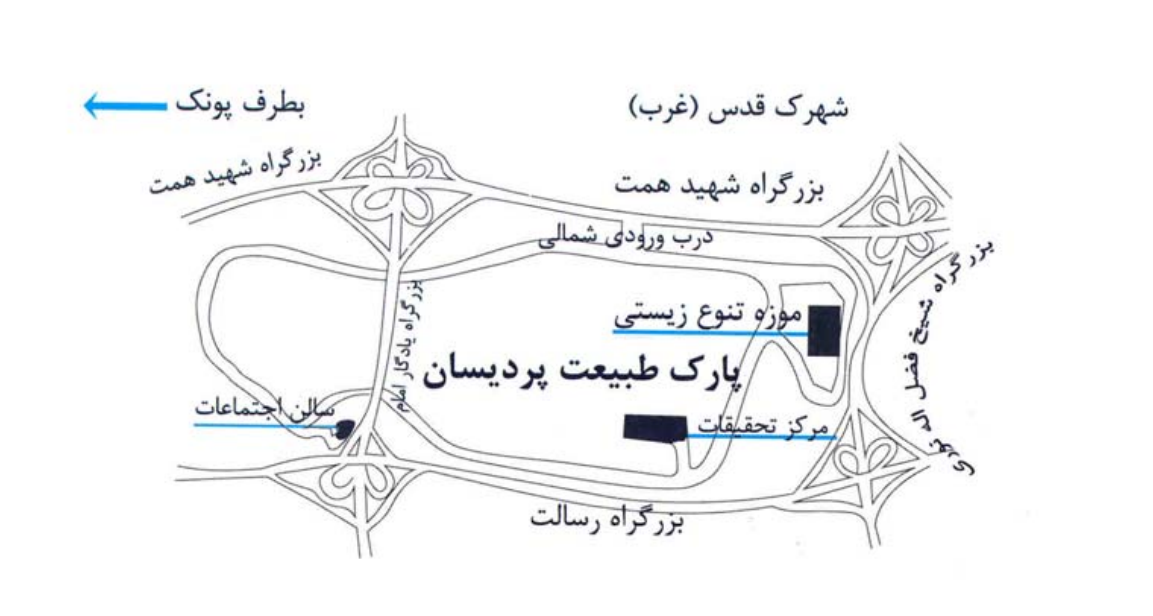
\includegraphics[scale = 0.5]{images/map.PNG}
    \caption{موقعیت موزه تنوع زیستی روی نقشه}
\end{figure}

بطور كلي سازمان آموزش و پرورش استان تهران با هماهنگي مديريت موزه اقدام به بازديدهاي گروهي دانش
آموزان بالاخص در مقاطع ابتدايي و راهنمايي مي نمايد . علاوه بر اين نظر به قرار گرفتن اين موزه در پارك
طبيعت پرديسان ، افرادي كه به قصد تفرج و گذران اوقات فراغت خود به اين مكان مي آيند قادر به بازديد از
اين موزه مي باشند ، همجنين هنرمندان ، مخصوصا نقاشان كه علاقمند به طراحي از طبيعت و جانوران
هستند از اين نمايشگاه استفاده مي نمايند . فضاي داخلي غرفه هاي موزه تنوع زيستي با الهام از طبيعت ايران
،جهان و زيستگاههاي طبيعي جانوران طراحي و فضاسازي شده است

در موزه تنوع زيستي تقسيم بندي بر اساس سيستم قاره اي – زيسـتگاهي بـوده كـه نمونـه هـاي متعـددي در
زيستگاه هاي مربوطه عرضه شده اند و شامل غرفه هاي ذيل مي باشد:

% \begin{tabular*}{cc}
    \begin{itemize}    
        \item غرفه نمونه‌های منقرض شده ايران: شامل مجسمه ها ي شير ايراني و ببر خزري
        \item غرفه نمونه هاي كمياب ايران
        \item غرفه تنوع زيستي ايران
        \item غرفه تنوع زيستي جهان
        \item غرفه خليج فارس
        \item غرفه تونل زير دريايي خليج فارس
        \item غرفه درياي مازندران
        \item غرفه قاره آسيا
        \item غرفه قاره اروپا
        \item غرفه قاره آفريقا
        \item غرفه قاره آمريكا
        \item غرفه قاره اقيانوسيه
        \item غرفه زيستگاه قطب جنوب
    \end{itemize}
    \begin{itemize}
        \item قاب پوست ببر خزري: اين پوست متعلق به ببر خزري است كه در پارك ملي گلستان به سال 1329شكار شده است.
        \item قاب پروانه ها
        \item ويترين حشرات
        \item اسكلت فيل آسيايي
        \item ويترين سنگ و كانيهاي ايران
        \item ويترين نرمتنان
        \item ويترين فسيلهاي گياهي
        \item ويترين فسيلهاي بي مهرگان
        \item ويترين فسيلهاي ماهيان آب شيرين
        \item تابلوي بازسازي فسيل‌هاي مراغه
        \item ويترين فسيلهاي مهره داران مراغه
    \end{itemize}
% \end{tabular*}


\begin{figure}
    \label{fig2.2}
    \centering
    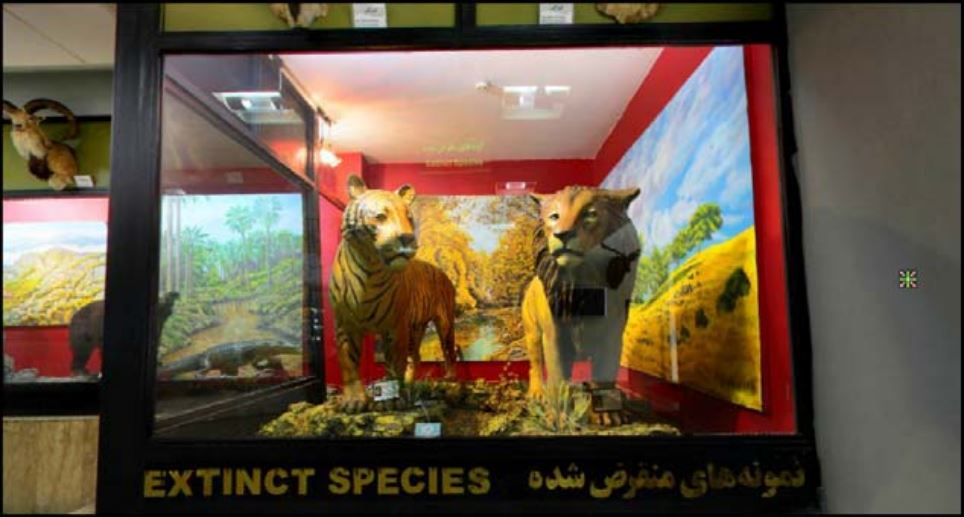
\includegraphics[scale = 0.45]{images/monqarez.jpg}
    \caption{دیورامای نمونه‌‌های منقرض شده}
\end{figure}

\subsection{کارگاه تاکسیدرمی}
نمونه هاي ارسالي در اين مكان ضمن فرايندهای پوست كنـي ، چربـي گيـري بـا مـواد شـيميايي
مختلف ، قالب سازي ، فرم دهي و پايه سازي تبديل به نمونه هاي نمايشي مي گردنـد.
	% the introduction section...

\chapter{سابقه‌ی تحقیق} \label{chapter:related-works}

\paragraph*{}

با ورود به عصر اطلاعات و پیشرفت بیوانفورماتیک و توالی یابی ژنتیکی، موزه های تنوع زیستی با داشتن گنجینه وسیعی و متنوعی از گونه های زیستی بسیار کمک کننده هستند.

\section{نقش موزه‌ها در حفظ تنوع زیستی}
منیتبذ
\subsection{گونه های در معرض انقراض}
شیبذ

\section{نقش موزه‌های تاریخ طبیعی در آموزش}
شیبذ


	% the proposed method section...

\chapter{روش پیشنهادی} \label{chapter:proposed-method}

\paragraph*{}
برای بررسی عملکرد موزه نیاز به مجموعه معیار هایی برای مقایسه داریم.


\section{بررسی موزه}
برای بررسی عملکرد موزه معیارهایی انتخاب می‌کنیم و در فصل بعد به مقایسه آن ها می‌پردازیم.

\subsection{ساختمان موزه}
اکثر موزه‌های داخل ایران درون ساختمان هایی که کاربری پیشینی متفاوتی داشتند برپا شدند. از جمله عمارت ها و کاخ های قدیمی.
بنابراین ویژگی‌های ساختمانی خاص مورد نیاز یک موزه را دارا نیستند.


\subsection{کامل بودن مجموعه}
موزه های تاریخ طبیعی شامل نمونه‌های جانوری، حشرات، آبزیان، گیاهان، فسیل‌ها و سنگ‌ها و کانی‌ها می‌شوند.


\subsection{نمونه‌ها}
یکی از عوامل منتخب برای ارزیابی، کیفیت نمونه‌هاست. بالا بودن کیفیت نمونه‌ها با شباهت به نمونه زنده مشخص می‌شود. این مسئله در کنار افزایش دقت اطلاعاتی که ببینده ارائه می‌کند، باعث جذابیت بیشتر بازدید از موزه می‌شود. 


\subsection{دیوراماها}
نمونه‌های تاکسیدرمی شده، در دیوراماها به نمایش گذاشته می‌شوند. ممکن است به چند گونه که زیست بوم مشترکی دارند یک دیوراما اختصاص داده شود.

دیوراماها با تصاویری از زیست بوم گونه آراسته می‌شوند. تصاویر باید ویژگی های معرف آن زیست بوم را داشته باشند و در معرفی اقلیم دقت داشته باشند. ممکن است از پوشش گیاهی آن زیست بوم نیز استفاده شود.

\subsection{نورپردازی}



\section{بررسی فعالیت‌ها}

\subsection{فعالیت‌های آموزشی}
نسبت به جمعیت سایر بازدید کنندگان، دانش آموزان از مخاطبان اصلی موزه هستند. معمولا بواسطه اردوهای آموزشی مدارس بازدید گروهی برایشان ترتیب داده می‌شود.
با توجه به مجهز بودن موزه به دپارتمان آموزش، این امر از اهداف اصلی موزه می‌باشد. 





	% the introduction section...

% \chapter{ارزیابی} \label{chapter:evaluation}

\paragraph*{}
داده‌های استفاده شده در این بخش توسط پژوهش میدانی انجام شده در تابستان 1401 بدست آمده‌است.
ابتدا به بررسی خود موزه و کیفیت موزه میپردازیم.
سپس به براساس اهداف و فعالیت هایی که از موزه معرفی کردیم مقایسه می‌کنیم.

\section*{بررسی موزه}

\subsection*{ساختمان موزه}
ساختمان موزه به هدف بهربرداری موزه طراحی شده است. نقشه آن شکل سنجاقک است.

\section*{نورپردازی}


\subsection*{کیفیت نمونه‌ها}

با توجه به تنوع جهان شمول نمونه‌های موزه، حفظ کیفیت تمام بخش‌ها به علت دسترسی نداشتن به نمونه‌های جدید سخت است. اما حتی اکثر نمونه‌های تاکسیدرمی شده از اکوسیستم بومی  متعلق به دهه 50 و 60 شمسی می‌باشند. قعالیت کارگاه تاکسیدرمی به مربوط به گونه‌های کمی ‌می‌شود و شیوه مدیریت این مسئله مانعی برای جذابیت های بالقوه موزه است.

\subsection*{کیفیت دیوراماها}

نکات فنی در طراحی دیوراماها به خوبی رعایت شده بود اما تصاویر دکور با کیفیت نقاشی دکور ها اکثرا پشم نوار نبود.
نمونه‌های گیاهی در تمام دیوراماها بلااستثنا خشک شده‌بودند.
نمونه های فسیلی فضای کافی نداشتند.
تابلوی پوست آخرین ببر ایرانی، مانند اضافه جهیزیه در خانه‌ای در مرحله خانه‌تکانی گوشه‌ای افتاده بود.
	% the conclusion section...

\chapter{نتیجه‌گیری} \label{chapter:conclusion}

\paragraph*{}
این فصل نتیجه‌گیری است.

	% the references section...
\bibliographystyle{plain-fa}
\renewcommand\bibname{فهرست مراجع}
\begin{thebibliography}{9} \label{chapter:references}


	\bibitem{naturalgroup} سند معرفی گروه موزه تاریخ طبیعی و تنوع زیستی
	\bibitem{hamshahri98} گزارش همشهری دوشنبه 21 بهمن 1398 کد مطلب :  94823 \url{https://newspaper.hamshahrionline.ir/id/94823/%D9%85%D8%AE%D8%B2%D9%86-%D8%AA%D8%A7%D8%B1%DB%8C%D8%AE-%D8%B7%D8%A8%DB%8C%D8%B9%DB%8C-%D8%A7%DB%8C%D8%B1%D8%A7%D9%86-11%D8%B3%D8%A7%D9%84-%DA%AF%D8%B4%D9%88%D8%AF%D9%87.html}
	\bibitem{ut98}  گزارش سایت دانشگاه تهران برای روز جهانی موزه سال 98 \url{https://science.ut.ac.ir/-/%D8%A8%D9%87-%D9%85%D9%86%D8%A7%D8%B3%D8%A8%D8%AA-%D8%B1%D9%88%D8%B2-%D8%AC%D9%87%D8%A7%D9%86%DB%8C-%D9%85%D9%88%D8%B2%D9%87-%D9%86%DA%AF%D8%A7%D9%87%DB%8C-%D8%A7%D8%AC%D9%85%D8%A7%D9%84%DB%8C-%D8%A8%D9%87-%D9%85%D9%88%D8%B2%D9%87-%D8%AA%D8%A7%D8%B1%DB%8C%D8%AE-%D8%B7%D8%A8%DB%8C%D8%B9%DB%8C-%D9%BE%D8%B1%D8%AF%DB%8C%D8%B3-%D8%B9%D9%84%D9%88%D9%85-%D8%AF%D8%A7%D9%86%D8%B4%DA%AF%D8%A7%D9%87-%D8%AA%D9%87%D8%B1%D8%A7%D9%86}
	\bibitem{inbook}
	\bibitem{inporceedings}


\end{thebibliography}
	
	% appendixes section...
	\begin {latin}
		% english abstract page...
		% english abstract section...

\chapter*{Abstract}

\paragraph*{}
This is the abstract in latin.

\subsection*{Keywords:}
Distributed Database System, Shared-Nothing, Distributed Databases, Incremental Repartitioning, Data Migration
		
		% english cover page...
		% remove page style from this specific page...
\thispagestyle{empty}

% begin the title...
\begin{center}
	% add the logo...
	
\includegraphics[scale=1.5]{logo}
	\mediumGap
	% report title...
	\huge \href{\universityLink}{\universityTitleLatin}
	\smallGap
	% university title...
	\large (\universitySubTitleLatin)
	\smallGap
	% department title...
	\Large \href{\departementLink}{\departementLatin}
	\bigGap
	% report type...
	\Large \reportTypeLatin
	\smallGap
	% field of study...
	\Large \fieldLatin Field
	\bigGap
	% report title...
	\large Title
	\smallGap
	\reportTitleLatin
	\bigGap
	% author information...
	\large By
	\smallGap
	\Large \href{\reportAuthorLink}{\reportAuthorLatin}
	\bigGap
	% instructor information...
	\large Supervisor
	\smallGap
	\Large \instructorLatin
	\bigGap
	% referees informations...
	\isDefined {\refereeFirstLatin} {
		% if first referee is defined then...
		\large Jury
		\smallGap
		\Large \refereeFirstLatin
		\isDefined {\refereeSecondLatin} {
			% if second referee is defined then...
			\smallGap
			\Large \refereeSecondLatin
		} {} % else is empty...
		\bigGap
	} {} % else is empty...
	\normalsize \reportDateLatin
\end{center}

	\end {latin}

\end {document}
